	\chapter{Ergebnisse}
	\label{chap:ergebnisse}
	
	Zuerst wird sichergestellt, dass das Programm sowohl bei paralleler als auch bei serieller Ausführung das gleiche Verhalten aufweist. Wie man an Bild \ref{fig:vergleichham} sieht, ist das der Fall, die Ergebnisse liegen aufeinander und sind insbesondere in ihren Fehlergrenzen gleich.
	
	\begin{figure}[htbp]
		% GNUPLOT: LaTeX picture with Postscript
\begingroup
  \makeatletter
  \providecommand\color[2][]{%
    \GenericError{(gnuplot) \space\space\space\@spaces}{%
      Package color not loaded in conjunction with
      terminal option `colourtext'%
    }{See the gnuplot documentation for explanation.%
    }{Either use 'blacktext' in gnuplot or load the package
      color.sty in LaTeX.}%
    \renewcommand\color[2][]{}%
  }%
  \providecommand\includegraphics[2][]{%
    \GenericError{(gnuplot) \space\space\space\@spaces}{%
      Package graphicx or graphics not loaded%
    }{See the gnuplot documentation for explanation.%
    }{The gnuplot epslatex terminal needs graphicx.sty or graphics.sty.}%
    \renewcommand\includegraphics[2][]{}%
  }%
  \providecommand\rotatebox[2]{#2}%
  \@ifundefined{ifGPcolor}{%
    \newif\ifGPcolor
    \GPcolortrue
  }{}%
  \@ifundefined{ifGPblacktext}{%
    \newif\ifGPblacktext
    \GPblacktextfalse
  }{}%
  % define a \g@addto@macro without @ in the name:
  \let\gplgaddtomacro\g@addto@macro
  % define empty templates for all commands taking text:
  \gdef\gplbacktext{}%
  \gdef\gplfronttext{}%
  \makeatother
  \ifGPblacktext
    % no textcolor at all
    \def\colorrgb#1{}%
    \def\colorgray#1{}%
  \else
    % gray or color?
    \ifGPcolor
      \def\colorrgb#1{\color[rgb]{#1}}%
      \def\colorgray#1{\color[gray]{#1}}%
      \expandafter\def\csname LTw\endcsname{\color{white}}%
      \expandafter\def\csname LTb\endcsname{\color{black}}%
      \expandafter\def\csname LTa\endcsname{\color{black}}%
      \expandafter\def\csname LT0\endcsname{\color[rgb]{1,0,0}}%
      \expandafter\def\csname LT1\endcsname{\color[rgb]{0,1,0}}%
      \expandafter\def\csname LT2\endcsname{\color[rgb]{0,0,1}}%
      \expandafter\def\csname LT3\endcsname{\color[rgb]{1,0,1}}%
      \expandafter\def\csname LT4\endcsname{\color[rgb]{0,1,1}}%
      \expandafter\def\csname LT5\endcsname{\color[rgb]{1,1,0}}%
      \expandafter\def\csname LT6\endcsname{\color[rgb]{0,0,0}}%
      \expandafter\def\csname LT7\endcsname{\color[rgb]{1,0.3,0}}%
      \expandafter\def\csname LT8\endcsname{\color[rgb]{0.5,0.5,0.5}}%
    \else
      % gray
      \def\colorrgb#1{\color{black}}%
      \def\colorgray#1{\color[gray]{#1}}%
      \expandafter\def\csname LTw\endcsname{\color{white}}%
      \expandafter\def\csname LTb\endcsname{\color{black}}%
      \expandafter\def\csname LTa\endcsname{\color{black}}%
      \expandafter\def\csname LT0\endcsname{\color{black}}%
      \expandafter\def\csname LT1\endcsname{\color{black}}%
      \expandafter\def\csname LT2\endcsname{\color{black}}%
      \expandafter\def\csname LT3\endcsname{\color{black}}%
      \expandafter\def\csname LT4\endcsname{\color{black}}%
      \expandafter\def\csname LT5\endcsname{\color{black}}%
      \expandafter\def\csname LT6\endcsname{\color{black}}%
      \expandafter\def\csname LT7\endcsname{\color{black}}%
      \expandafter\def\csname LT8\endcsname{\color{black}}%
    \fi
  \fi
    \setlength{\unitlength}{0.0500bp}%
    \ifx\gptboxheight\undefined%
      \newlength{\gptboxheight}%
      \newlength{\gptboxwidth}%
      \newsavebox{\gptboxtext}%
    \fi%
    \setlength{\fboxrule}{0.5pt}%
    \setlength{\fboxsep}{1pt}%
\begin{picture}(8640.00,6480.00)%
    \gplgaddtomacro\gplbacktext{%
      \csname LTb\endcsname%
      \put(946,704){\makebox(0,0)[r]{\strut{}$-2.2$}}%
      \put(946,1316){\makebox(0,0)[r]{\strut{}$-2$}}%
      \put(946,1929){\makebox(0,0)[r]{\strut{}$-1.8$}}%
      \put(946,2541){\makebox(0,0)[r]{\strut{}$-1.6$}}%
      \put(946,3153){\makebox(0,0)[r]{\strut{}$-1.4$}}%
      \put(946,3766){\makebox(0,0)[r]{\strut{}$-1.2$}}%
      \put(946,4378){\makebox(0,0)[r]{\strut{}$-1$}}%
      \put(946,4990){\makebox(0,0)[r]{\strut{}$-0.8$}}%
      \put(946,5603){\makebox(0,0)[r]{\strut{}$-0.6$}}%
      \put(946,6215){\makebox(0,0)[r]{\strut{}$-0.4$}}%
      \put(1078,484){\makebox(0,0){\strut{}$0$}}%
      \put(2511,484){\makebox(0,0){\strut{}$1$}}%
      \put(3944,484){\makebox(0,0){\strut{}$2$}}%
      \put(5377,484){\makebox(0,0){\strut{}$3$}}%
      \put(6810,484){\makebox(0,0){\strut{}$4$}}%
      \put(8243,484){\makebox(0,0){\strut{}$5$}}%
    }%
    \gplgaddtomacro\gplfronttext{%
      \csname LTb\endcsname%
      \put(176,3459){\rotatebox{-270}{\makebox(0,0){\strut{}$H/\text{laenge}^2$}}}%
      \put(4660,154){\makebox(0,0){\strut{}Temperatur}}%
      \csname LTb\endcsname%
      \put(4642,6042){\makebox(0,0)[r]{\strut{}zeilenweise durchgehen}}%
      \csname LTb\endcsname%
      \put(4642,5822){\makebox(0,0)[r]{\strut{}Schachbrettmuster parallel}}%
    }%
    \gplbacktext
    \put(0,0){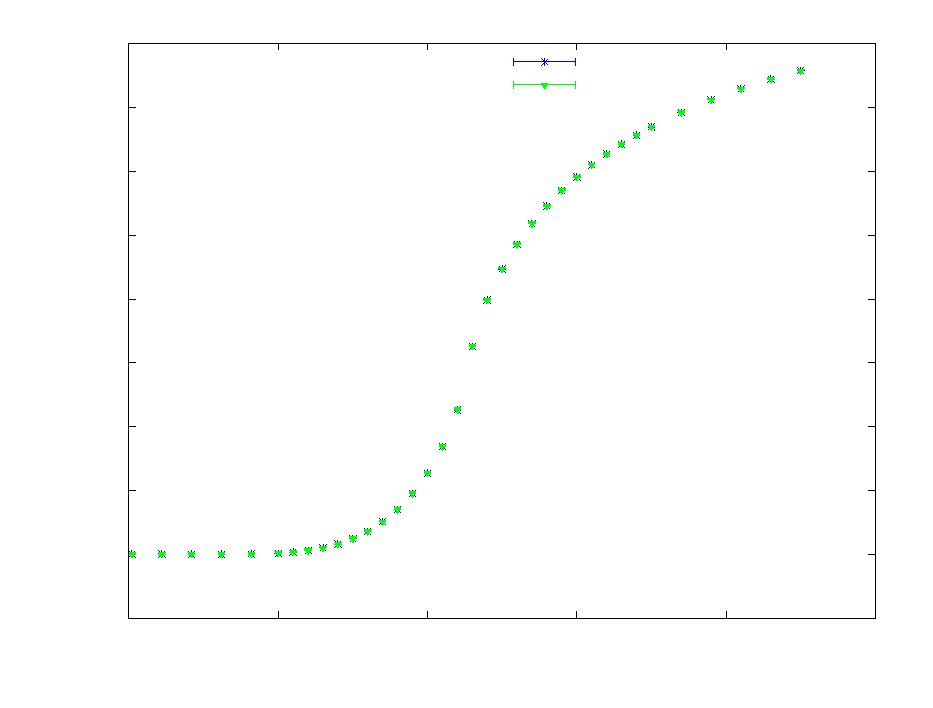
\includegraphics{vergleichham}}%
    \gplfronttext
  \end{picture}%
\endgroup

		\caption[Hamiltonian mit und ohne Parallelisierung]{Hamiltonian mit und ohne Parallelisierung bei verschiedenen Temperaturen gemessen. Die Fehler sind mit Blocklänge 128 bestimmt und so klein, dass sie fast nicht sichtbar sind.}
		\label{fig:vergleichham}
	\end{figure}
	
	Um zu ermitteln, mit wie vielen Cores idealerweise gemessen werden sollte, wurde die Skalierung der sweep-Funktion betrachtet. Hierbei wurde für verschiedene Gitterlängen und Temperaturen die Zeit, die für 10.000 Ausführungen der sweep-Funktion benötigt wurde, gemessen. 
	
	Wie man an Bild sieht, ist die Parallelisierung für kleine Gitterlängen sinnlos, es wird nur mehr overhead eingeführt und die benötigte Zeit steigt mit Anzahl der Cores.
	
	Ab einer gewissen Gitterlänge sinkt die benötigte Rechenzeit mit mehr Cores, sinkt allerdings für mehr Cores, wenn es mehr Overhead gibt. Bei steigender Gitterlänge wird allerdings auch die Laufzeitverbesserung für mehr Cores sichtbar, es bildet sich erst ein Plateau, was für lange Gitterlängen schließlich in eine monoton steigende Funktion übergeht.
	
	Wenn man sich die Skalierung bei verschiedenen Temperaturen anguckt, gibt es auch hier Unterschiede bei konstanter Gitterlänge: für niedrigere Temperaturen ist die Laufzeit geringer, allerdings der maximale speedup kleiner. Vermutlich kommt dies daher, dass bei niedrigen Temperaturen die Akzeptanzrate geringer ist und somit seltener eine Addition beim Hamiltonian durchgeführt werden muss.
	
	Bei Gitterlängen ab  entspricht das Ergebnis somit den Erwartungen aus Abschnitt \ref{subsec:openmptheorie}
	%Insgesamt entspricht somit die Skalierung bei hohen Gitterlängen dem Ahmdahlschen Gesetz.
	Messungen der Parallelisierung von messen/sweep auf lcpunode02 in QBiG: Bis zu 12 Kerne. Kennwerte von lcpunode02?
	%Parallelisierung Bootstrap?
	
	%Zuerst: Vergleich der verschiedenen sweep-Funktionen: Hamiltonian gleich. Bild.
	
	%Skalierung auf lcpunode2: Vergleich zwei Schleifen/tryflip/Temperaturen?
	%Bild von idealem Code, Skalierung wie erwartet (nach Ahmdahls law?)
	
	In Bild \ref{fig:ergebnisakzeptanzrate} ist die Akzeptanzrate als Funktion von der Temperatur dargestellt. Bei kleinen Temperaturen ist sie null, steigt ab ca. $T=1$ an, hat bei ca. $T=\num{2,2}$ einen Wendepunkt mit Akzeptanzrate ca. $\num{0,2}$ und nähert sich danach asymptotisch dem Wert $1$.
	
	\begin{figure}[htbp]
		% GNUPLOT: LaTeX picture with Postscript
\begingroup
  \makeatletter
  \providecommand\color[2][]{%
    \GenericError{(gnuplot) \space\space\space\@spaces}{%
      Package color not loaded in conjunction with
      terminal option `colourtext'%
    }{See the gnuplot documentation for explanation.%
    }{Either use 'blacktext' in gnuplot or load the package
      color.sty in LaTeX.}%
    \renewcommand\color[2][]{}%
  }%
  \providecommand\includegraphics[2][]{%
    \GenericError{(gnuplot) \space\space\space\@spaces}{%
      Package graphicx or graphics not loaded%
    }{See the gnuplot documentation for explanation.%
    }{The gnuplot epslatex terminal needs graphicx.sty or graphics.sty.}%
    \renewcommand\includegraphics[2][]{}%
  }%
  \providecommand\rotatebox[2]{#2}%
  \@ifundefined{ifGPcolor}{%
    \newif\ifGPcolor
    \GPcolortrue
  }{}%
  \@ifundefined{ifGPblacktext}{%
    \newif\ifGPblacktext
    \GPblacktextfalse
  }{}%
  % define a \g@addto@macro without @ in the name:
  \let\gplgaddtomacro\g@addto@macro
  % define empty templates for all commands taking text:
  \gdef\gplbacktext{}%
  \gdef\gplfronttext{}%
  \makeatother
  \ifGPblacktext
    % no textcolor at all
    \def\colorrgb#1{}%
    \def\colorgray#1{}%
  \else
    % gray or color?
    \ifGPcolor
      \def\colorrgb#1{\color[rgb]{#1}}%
      \def\colorgray#1{\color[gray]{#1}}%
      \expandafter\def\csname LTw\endcsname{\color{white}}%
      \expandafter\def\csname LTb\endcsname{\color{black}}%
      \expandafter\def\csname LTa\endcsname{\color{black}}%
      \expandafter\def\csname LT0\endcsname{\color[rgb]{1,0,0}}%
      \expandafter\def\csname LT1\endcsname{\color[rgb]{0,1,0}}%
      \expandafter\def\csname LT2\endcsname{\color[rgb]{0,0,1}}%
      \expandafter\def\csname LT3\endcsname{\color[rgb]{1,0,1}}%
      \expandafter\def\csname LT4\endcsname{\color[rgb]{0,1,1}}%
      \expandafter\def\csname LT5\endcsname{\color[rgb]{1,1,0}}%
      \expandafter\def\csname LT6\endcsname{\color[rgb]{0,0,0}}%
      \expandafter\def\csname LT7\endcsname{\color[rgb]{1,0.3,0}}%
      \expandafter\def\csname LT8\endcsname{\color[rgb]{0.5,0.5,0.5}}%
    \else
      % gray
      \def\colorrgb#1{\color{black}}%
      \def\colorgray#1{\color[gray]{#1}}%
      \expandafter\def\csname LTw\endcsname{\color{white}}%
      \expandafter\def\csname LTb\endcsname{\color{black}}%
      \expandafter\def\csname LTa\endcsname{\color{black}}%
      \expandafter\def\csname LT0\endcsname{\color{black}}%
      \expandafter\def\csname LT1\endcsname{\color{black}}%
      \expandafter\def\csname LT2\endcsname{\color{black}}%
      \expandafter\def\csname LT3\endcsname{\color{black}}%
      \expandafter\def\csname LT4\endcsname{\color{black}}%
      \expandafter\def\csname LT5\endcsname{\color{black}}%
      \expandafter\def\csname LT6\endcsname{\color{black}}%
      \expandafter\def\csname LT7\endcsname{\color{black}}%
      \expandafter\def\csname LT8\endcsname{\color{black}}%
    \fi
  \fi
    \setlength{\unitlength}{0.0500bp}%
    \ifx\gptboxheight\undefined%
      \newlength{\gptboxheight}%
      \newlength{\gptboxwidth}%
      \newsavebox{\gptboxtext}%
    \fi%
    \setlength{\fboxrule}{0.5pt}%
    \setlength{\fboxsep}{1pt}%
\begin{picture}(8640.00,4320.00)%
    \gplgaddtomacro\gplbacktext{%
      \csname LTb\endcsname%
      \put(1164,737){\makebox(0,0)[r]{\strut{}$0$}}%
      \put(1164,1394){\makebox(0,0)[r]{\strut{}$0.2$}}%
      \put(1164,2051){\makebox(0,0)[r]{\strut{}$0.4$}}%
      \put(1164,2708){\makebox(0,0)[r]{\strut{}$0.6$}}%
      \put(1164,3365){\makebox(0,0)[r]{\strut{}$0.8$}}%
      \put(1164,4022){\makebox(0,0)[r]{\strut{}$1$}}%
      \put(1299,484){\makebox(0,0){\strut{}$0$}}%
      \put(1990,484){\makebox(0,0){\strut{}$2000$}}%
      \put(2680,484){\makebox(0,0){\strut{}$4000$}}%
      \put(3370,484){\makebox(0,0){\strut{}$6000$}}%
      \put(4061,484){\makebox(0,0){\strut{}$8000$}}%
      \put(4751,484){\makebox(0,0){\strut{}$10000$}}%
    }%
    \gplgaddtomacro\gplfronttext{%
      \csname LTb\endcsname%
      \put(526,2379){\rotatebox{-270}{\makebox(0,0){\strut{}Akzeptanzrate}}}%
      \put(3023,154){\makebox(0,0){\strut{}Temperatur}}%
    }%
    \gplgaddtomacro\gplbacktext{%
      \csname LTb\endcsname%
      \put(4620,737){\makebox(0,0)[r]{\strut{}}}%
      \put(4620,1394){\makebox(0,0)[r]{\strut{}}}%
      \put(4620,2051){\makebox(0,0)[r]{\strut{}}}%
      \put(4620,2708){\makebox(0,0)[r]{\strut{}}}%
      \put(4620,3365){\makebox(0,0)[r]{\strut{}}}%
      \put(4620,4022){\makebox(0,0)[r]{\strut{}}}%
      \put(4752,484){\makebox(0,0){\strut{}$0$}}%
      \put(5443,484){\makebox(0,0){\strut{}$1$}}%
      \put(6134,484){\makebox(0,0){\strut{}$2$}}%
      \put(6825,484){\makebox(0,0){\strut{}$3$}}%
      \put(7516,484){\makebox(0,0){\strut{}$4$}}%
      \put(8207,484){\makebox(0,0){\strut{}$5$}}%
    }%
    \gplgaddtomacro\gplfronttext{%
      \csname LTb\endcsname%
      \put(6479,154){\makebox(0,0){\strut{}Temperatur}}%
    }%
    \gplbacktext
    \put(0,0){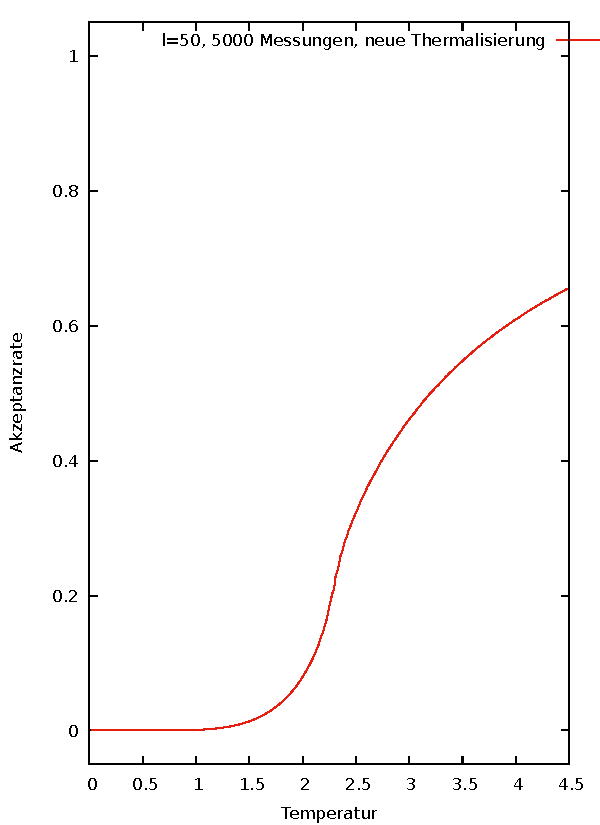
\includegraphics{akzeptanzrate}}%
    \gplfronttext
  \end{picture}%
\endgroup

		\caption[Akzeptanzrate in Abhängigkeit von der Temperatur]{Akzeptanzrate in Abhängigkeit von der Temperatur, gemessen bei Gitterlänge 120, mit Blocklänge 128 zur Fehlerberechnung. Die Fehler sind so klein, dass sie fast nicht sichtbar sind.}
		\label{fig:ergebnisakzeptanzrate}
	\end{figure}
	
	Der Hamiltonian verhält sich qualitativ ähnlich, siehe Bild \ref{fig:ergebnishamiltonian}. Bei geringen Temperaturen hat er den Wert $-2\cdot\text{laenge}^2$, was auf ein vollkommen homogen ausgerichtetes Gitter hinweist. Bei ca T=2,2 beträgt der Hamiltonian ca. $-\num{1,4}\cdot\text{laenge}^2$ und nähert sich dann asymptotisch null.
	
	\begin{figure}[htbp]
		% GNUPLOT: LaTeX picture with Postscript
\begingroup
  \makeatletter
  \providecommand\color[2][]{%
    \GenericError{(gnuplot) \space\space\space\@spaces}{%
      Package color not loaded in conjunction with
      terminal option `colourtext'%
    }{See the gnuplot documentation for explanation.%
    }{Either use 'blacktext' in gnuplot or load the package
      color.sty in LaTeX.}%
    \renewcommand\color[2][]{}%
  }%
  \providecommand\includegraphics[2][]{%
    \GenericError{(gnuplot) \space\space\space\@spaces}{%
      Package graphicx or graphics not loaded%
    }{See the gnuplot documentation for explanation.%
    }{The gnuplot epslatex terminal needs graphicx.sty or graphics.sty.}%
    \renewcommand\includegraphics[2][]{}%
  }%
  \providecommand\rotatebox[2]{#2}%
  \@ifundefined{ifGPcolor}{%
    \newif\ifGPcolor
    \GPcolortrue
  }{}%
  \@ifundefined{ifGPblacktext}{%
    \newif\ifGPblacktext
    \GPblacktextfalse
  }{}%
  % define a \g@addto@macro without @ in the name:
  \let\gplgaddtomacro\g@addto@macro
  % define empty templates for all commands taking text:
  \gdef\gplbacktext{}%
  \gdef\gplfronttext{}%
  \makeatother
  \ifGPblacktext
    % no textcolor at all
    \def\colorrgb#1{}%
    \def\colorgray#1{}%
  \else
    % gray or color?
    \ifGPcolor
      \def\colorrgb#1{\color[rgb]{#1}}%
      \def\colorgray#1{\color[gray]{#1}}%
      \expandafter\def\csname LTw\endcsname{\color{white}}%
      \expandafter\def\csname LTb\endcsname{\color{black}}%
      \expandafter\def\csname LTa\endcsname{\color{black}}%
      \expandafter\def\csname LT0\endcsname{\color[rgb]{1,0,0}}%
      \expandafter\def\csname LT1\endcsname{\color[rgb]{0,1,0}}%
      \expandafter\def\csname LT2\endcsname{\color[rgb]{0,0,1}}%
      \expandafter\def\csname LT3\endcsname{\color[rgb]{1,0,1}}%
      \expandafter\def\csname LT4\endcsname{\color[rgb]{0,1,1}}%
      \expandafter\def\csname LT5\endcsname{\color[rgb]{1,1,0}}%
      \expandafter\def\csname LT6\endcsname{\color[rgb]{0,0,0}}%
      \expandafter\def\csname LT7\endcsname{\color[rgb]{1,0.3,0}}%
      \expandafter\def\csname LT8\endcsname{\color[rgb]{0.5,0.5,0.5}}%
    \else
      % gray
      \def\colorrgb#1{\color{black}}%
      \def\colorgray#1{\color[gray]{#1}}%
      \expandafter\def\csname LTw\endcsname{\color{white}}%
      \expandafter\def\csname LTb\endcsname{\color{black}}%
      \expandafter\def\csname LTa\endcsname{\color{black}}%
      \expandafter\def\csname LT0\endcsname{\color{black}}%
      \expandafter\def\csname LT1\endcsname{\color{black}}%
      \expandafter\def\csname LT2\endcsname{\color{black}}%
      \expandafter\def\csname LT3\endcsname{\color{black}}%
      \expandafter\def\csname LT4\endcsname{\color{black}}%
      \expandafter\def\csname LT5\endcsname{\color{black}}%
      \expandafter\def\csname LT6\endcsname{\color{black}}%
      \expandafter\def\csname LT7\endcsname{\color{black}}%
      \expandafter\def\csname LT8\endcsname{\color{black}}%
    \fi
  \fi
    \setlength{\unitlength}{0.0500bp}%
    \ifx\gptboxheight\undefined%
      \newlength{\gptboxheight}%
      \newlength{\gptboxwidth}%
      \newsavebox{\gptboxtext}%
    \fi%
    \setlength{\fboxrule}{0.5pt}%
    \setlength{\fboxsep}{1pt}%
\begin{picture}(8640.00,4320.00)%
    \gplgaddtomacro\gplbacktext{%
      \csname LTb\endcsname%
      \put(1164,721){\makebox(0,0)[r]{\strut{}$-2$}}%
      \put(1164,1550){\makebox(0,0)[r]{\strut{}$-1.5$}}%
      \put(1164,2380){\makebox(0,0)[r]{\strut{}$-1$}}%
      \put(1164,3209){\makebox(0,0)[r]{\strut{}$-0.5$}}%
      \put(1164,4038){\makebox(0,0)[r]{\strut{}$0$}}%
      \put(1299,484){\makebox(0,0){\strut{}$0$}}%
      \put(1990,484){\makebox(0,0){\strut{}$2000$}}%
      \put(2680,484){\makebox(0,0){\strut{}$4000$}}%
      \put(3370,484){\makebox(0,0){\strut{}$6000$}}%
      \put(4061,484){\makebox(0,0){\strut{}$8000$}}%
      \put(4751,484){\makebox(0,0){\strut{}$10000$}}%
    }%
    \gplgaddtomacro\gplfronttext{%
      \csname LTb\endcsname%
      \put(394,2379){\rotatebox{-270}{\makebox(0,0){\strut{}$H/\text{laenge}^2$}}}%
      \put(3023,154){\makebox(0,0){\strut{}Temperatur}}%
    }%
    \gplgaddtomacro\gplbacktext{%
      \csname LTb\endcsname%
      \put(4620,721){\makebox(0,0)[r]{\strut{}}}%
      \put(4620,1550){\makebox(0,0)[r]{\strut{}}}%
      \put(4620,2380){\makebox(0,0)[r]{\strut{}}}%
      \put(4620,3209){\makebox(0,0)[r]{\strut{}}}%
      \put(4620,4038){\makebox(0,0)[r]{\strut{}}}%
      \put(4752,484){\makebox(0,0){\strut{}$0$}}%
      \put(5443,484){\makebox(0,0){\strut{}$1$}}%
      \put(6134,484){\makebox(0,0){\strut{}$2$}}%
      \put(6825,484){\makebox(0,0){\strut{}$3$}}%
      \put(7516,484){\makebox(0,0){\strut{}$4$}}%
      \put(8207,484){\makebox(0,0){\strut{}$5$}}%
    }%
    \gplgaddtomacro\gplfronttext{%
      \csname LTb\endcsname%
      \put(6479,154){\makebox(0,0){\strut{}Temperatur}}%
    }%
    \gplbacktext
    \put(0,0){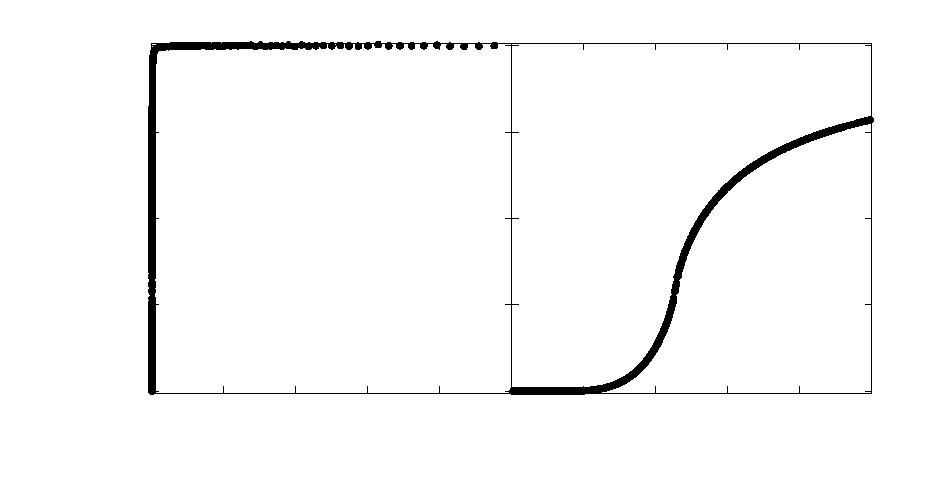
\includegraphics{hamiltonian}}%
    \gplfronttext
  \end{picture}%
\endgroup

		\caption[Hamiltonian in Abhängigkeit von der Temperatur]{Hamiltonian in Abhängigkeit von der Temperatur, gemessen bei Gitterlänge 120, mit Blocklänge 128 zur Fehlerberechnung. Die Fehler sind so klein, dass sie fast nicht sichtbar sind.}
		\label{fig:ergebnishamiltonian}
	\end{figure}
	
%	Dann Akzeptanzrate von wo bis wo, mit gebootstraptem Fehler? Geht auf 1 hoch?
%	\begin{verbatim}
%	test
%	\end{verbatim}

	Die Magnetisierung verhält sich wie nach Gl. \ref{eq:magnetisierungsgleichungliteratur} erwartet: Bei geringen Temperaturen ist sie eins, danach wird sich kleiner. Bei ca. $\num{2,2}$ hat sie einen starken Abfall, und nähert sich danach einem konstanten Wert größer als null an. Nach Gl. \ref{eq:magnetisierungsgleichungliteratur} wäre zu erwarten, dass der Abfall eine scharfe Kante bildet und danach die Magnetisierung null ist, dies ist allerdings aufgrund der endlichen Gittergöße nicht der Fall, wie in \cite[Abschnitt 2.3.3]{binderheermann} erläutert wird.

	
	\begin{figure}[htbp]
		% GNUPLOT: LaTeX picture with Postscript
\begingroup
  \makeatletter
  \providecommand\color[2][]{%
    \GenericError{(gnuplot) \space\space\space\@spaces}{%
      Package color not loaded in conjunction with
      terminal option `colourtext'%
    }{See the gnuplot documentation for explanation.%
    }{Either use 'blacktext' in gnuplot or load the package
      color.sty in LaTeX.}%
    \renewcommand\color[2][]{}%
  }%
  \providecommand\includegraphics[2][]{%
    \GenericError{(gnuplot) \space\space\space\@spaces}{%
      Package graphicx or graphics not loaded%
    }{See the gnuplot documentation for explanation.%
    }{The gnuplot epslatex terminal needs graphicx.sty or graphics.sty.}%
    \renewcommand\includegraphics[2][]{}%
  }%
  \providecommand\rotatebox[2]{#2}%
  \@ifundefined{ifGPcolor}{%
    \newif\ifGPcolor
    \GPcolortrue
  }{}%
  \@ifundefined{ifGPblacktext}{%
    \newif\ifGPblacktext
    \GPblacktextfalse
  }{}%
  % define a \g@addto@macro without @ in the name:
  \let\gplgaddtomacro\g@addto@macro
  % define empty templates for all commands taking text:
  \gdef\gplbacktext{}%
  \gdef\gplfronttext{}%
  \makeatother
  \ifGPblacktext
    % no textcolor at all
    \def\colorrgb#1{}%
    \def\colorgray#1{}%
  \else
    % gray or color?
    \ifGPcolor
      \def\colorrgb#1{\color[rgb]{#1}}%
      \def\colorgray#1{\color[gray]{#1}}%
      \expandafter\def\csname LTw\endcsname{\color{white}}%
      \expandafter\def\csname LTb\endcsname{\color{black}}%
      \expandafter\def\csname LTa\endcsname{\color{black}}%
      \expandafter\def\csname LT0\endcsname{\color[rgb]{1,0,0}}%
      \expandafter\def\csname LT1\endcsname{\color[rgb]{0,1,0}}%
      \expandafter\def\csname LT2\endcsname{\color[rgb]{0,0,1}}%
      \expandafter\def\csname LT3\endcsname{\color[rgb]{1,0,1}}%
      \expandafter\def\csname LT4\endcsname{\color[rgb]{0,1,1}}%
      \expandafter\def\csname LT5\endcsname{\color[rgb]{1,1,0}}%
      \expandafter\def\csname LT6\endcsname{\color[rgb]{0,0,0}}%
      \expandafter\def\csname LT7\endcsname{\color[rgb]{1,0.3,0}}%
      \expandafter\def\csname LT8\endcsname{\color[rgb]{0.5,0.5,0.5}}%
    \else
      % gray
      \def\colorrgb#1{\color{black}}%
      \def\colorgray#1{\color[gray]{#1}}%
      \expandafter\def\csname LTw\endcsname{\color{white}}%
      \expandafter\def\csname LTb\endcsname{\color{black}}%
      \expandafter\def\csname LTa\endcsname{\color{black}}%
      \expandafter\def\csname LT0\endcsname{\color{black}}%
      \expandafter\def\csname LT1\endcsname{\color{black}}%
      \expandafter\def\csname LT2\endcsname{\color{black}}%
      \expandafter\def\csname LT3\endcsname{\color{black}}%
      \expandafter\def\csname LT4\endcsname{\color{black}}%
      \expandafter\def\csname LT5\endcsname{\color{black}}%
      \expandafter\def\csname LT6\endcsname{\color{black}}%
      \expandafter\def\csname LT7\endcsname{\color{black}}%
      \expandafter\def\csname LT8\endcsname{\color{black}}%
    \fi
  \fi
    \setlength{\unitlength}{0.0500bp}%
    \ifx\gptboxheight\undefined%
      \newlength{\gptboxheight}%
      \newlength{\gptboxwidth}%
      \newsavebox{\gptboxtext}%
    \fi%
    \setlength{\fboxrule}{0.5pt}%
    \setlength{\fboxsep}{1pt}%
\begin{picture}(8640.00,4320.00)%
    \gplgaddtomacro\gplbacktext{%
      \csname LTb\endcsname%
      \put(1164,737){\makebox(0,0)[r]{\strut{}$0$}}%
      \put(1164,1394){\makebox(0,0)[r]{\strut{}$0.2$}}%
      \put(1164,2051){\makebox(0,0)[r]{\strut{}$0.4$}}%
      \put(1164,2708){\makebox(0,0)[r]{\strut{}$0.6$}}%
      \put(1164,3365){\makebox(0,0)[r]{\strut{}$0.8$}}%
      \put(1164,4022){\makebox(0,0)[r]{\strut{}$1$}}%
      \put(1299,484){\makebox(0,0){\strut{}$0$}}%
      \put(1990,484){\makebox(0,0){\strut{}$2000$}}%
      \put(2680,484){\makebox(0,0){\strut{}$4000$}}%
      \put(3370,484){\makebox(0,0){\strut{}$6000$}}%
      \put(4061,484){\makebox(0,0){\strut{}$8000$}}%
      \put(4751,484){\makebox(0,0){\strut{}$10000$}}%
    }%
    \gplgaddtomacro\gplfronttext{%
      \csname LTb\endcsname%
      \put(526,2379){\rotatebox{-270}{\makebox(0,0){\strut{}$M$}}}%
      \put(3023,154){\makebox(0,0){\strut{}Temperatur}}%
    }%
    \gplgaddtomacro\gplbacktext{%
      \csname LTb\endcsname%
      \put(4620,737){\makebox(0,0)[r]{\strut{}}}%
      \put(4620,1394){\makebox(0,0)[r]{\strut{}}}%
      \put(4620,2051){\makebox(0,0)[r]{\strut{}}}%
      \put(4620,2708){\makebox(0,0)[r]{\strut{}}}%
      \put(4620,3365){\makebox(0,0)[r]{\strut{}}}%
      \put(4620,4022){\makebox(0,0)[r]{\strut{}}}%
      \put(4752,484){\makebox(0,0){\strut{}$0$}}%
      \put(5443,484){\makebox(0,0){\strut{}$1$}}%
      \put(6134,484){\makebox(0,0){\strut{}$2$}}%
      \put(6825,484){\makebox(0,0){\strut{}$3$}}%
      \put(7516,484){\makebox(0,0){\strut{}$4$}}%
      \put(8207,484){\makebox(0,0){\strut{}$5$}}%
    }%
    \gplgaddtomacro\gplfronttext{%
      \csname LTb\endcsname%
      \put(6479,154){\makebox(0,0){\strut{}Temperatur}}%
    }%
    \gplbacktext
    \put(0,0){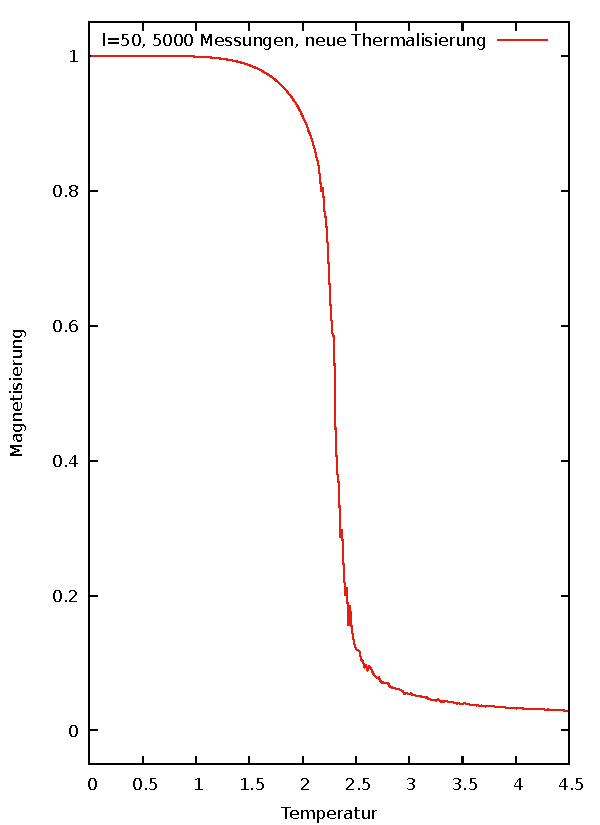
\includegraphics{magnetisierung}}%
    \gplfronttext
  \end{picture}%
\endgroup

		\caption[Magnetisierung in Abhängigkeit von der Temperatur]{Magnetisierung in Abhängigkeit von der Temperatur, gemessen bei Gitterlänge 120, mit Blocklänge 128 zur Fehlerberechnung. Die Fehler sind teilweise so klein, dass sie fast nicht sichtbar sind.}
		\label{fig:ergebnismagnetisierung}
	\end{figure}	
	
	%Dann Magnetisierung: Vergleich zweier Längen, Erklärung finite size Effekts wie in Binder-Heermann erwähnt.
	In Bild \ref{fig:ergebnismagnetisierung} ist dieses Verhalten zu sehen. In Bild \ref{fig:maglaenge} ist dies noch deutlicher zu sehen, dort wird die Magnetisierung bei zwei verschiedenen Längen miteinander verglichen. Es fällt auf, dass bei kleineren Längen der Abfall der Magnetisierung weniger steil ist, sowie die Magnetisierung oberhalb des kritischen Punktes einen größeren Wert hat. Auch dies deckt sich mit den Erwartungen aus \cite[Abschnitt 2.3.3]{binderheermann}.%, ebenso wie der Vergleich zweier Längen: bei kleineren Gitterlängen ist der Abfall weniger steil und der Wert der Magnetisierung bei hohen Temperaturen größer.
	
	
	\begin{figure}[htbp]
		% GNUPLOT: LaTeX picture with Postscript
\begingroup
  \makeatletter
  \providecommand\color[2][]{%
    \GenericError{(gnuplot) \space\space\space\@spaces}{%
      Package color not loaded in conjunction with
      terminal option `colourtext'%
    }{See the gnuplot documentation for explanation.%
    }{Either use 'blacktext' in gnuplot or load the package
      color.sty in LaTeX.}%
    \renewcommand\color[2][]{}%
  }%
  \providecommand\includegraphics[2][]{%
    \GenericError{(gnuplot) \space\space\space\@spaces}{%
      Package graphicx or graphics not loaded%
    }{See the gnuplot documentation for explanation.%
    }{The gnuplot epslatex terminal needs graphicx.sty or graphics.sty.}%
    \renewcommand\includegraphics[2][]{}%
  }%
  \providecommand\rotatebox[2]{#2}%
  \@ifundefined{ifGPcolor}{%
    \newif\ifGPcolor
    \GPcolortrue
  }{}%
  \@ifundefined{ifGPblacktext}{%
    \newif\ifGPblacktext
    \GPblacktextfalse
  }{}%
  % define a \g@addto@macro without @ in the name:
  \let\gplgaddtomacro\g@addto@macro
  % define empty templates for all commands taking text:
  \gdef\gplbacktext{}%
  \gdef\gplfronttext{}%
  \makeatother
  \ifGPblacktext
    % no textcolor at all
    \def\colorrgb#1{}%
    \def\colorgray#1{}%
  \else
    % gray or color?
    \ifGPcolor
      \def\colorrgb#1{\color[rgb]{#1}}%
      \def\colorgray#1{\color[gray]{#1}}%
      \expandafter\def\csname LTw\endcsname{\color{white}}%
      \expandafter\def\csname LTb\endcsname{\color{black}}%
      \expandafter\def\csname LTa\endcsname{\color{black}}%
      \expandafter\def\csname LT0\endcsname{\color[rgb]{1,0,0}}%
      \expandafter\def\csname LT1\endcsname{\color[rgb]{0,1,0}}%
      \expandafter\def\csname LT2\endcsname{\color[rgb]{0,0,1}}%
      \expandafter\def\csname LT3\endcsname{\color[rgb]{1,0,1}}%
      \expandafter\def\csname LT4\endcsname{\color[rgb]{0,1,1}}%
      \expandafter\def\csname LT5\endcsname{\color[rgb]{1,1,0}}%
      \expandafter\def\csname LT6\endcsname{\color[rgb]{0,0,0}}%
      \expandafter\def\csname LT7\endcsname{\color[rgb]{1,0.3,0}}%
      \expandafter\def\csname LT8\endcsname{\color[rgb]{0.5,0.5,0.5}}%
    \else
      % gray
      \def\colorrgb#1{\color{black}}%
      \def\colorgray#1{\color[gray]{#1}}%
      \expandafter\def\csname LTw\endcsname{\color{white}}%
      \expandafter\def\csname LTb\endcsname{\color{black}}%
      \expandafter\def\csname LTa\endcsname{\color{black}}%
      \expandafter\def\csname LT0\endcsname{\color{black}}%
      \expandafter\def\csname LT1\endcsname{\color{black}}%
      \expandafter\def\csname LT2\endcsname{\color{black}}%
      \expandafter\def\csname LT3\endcsname{\color{black}}%
      \expandafter\def\csname LT4\endcsname{\color{black}}%
      \expandafter\def\csname LT5\endcsname{\color{black}}%
      \expandafter\def\csname LT6\endcsname{\color{black}}%
      \expandafter\def\csname LT7\endcsname{\color{black}}%
      \expandafter\def\csname LT8\endcsname{\color{black}}%
    \fi
  \fi
    \setlength{\unitlength}{0.0500bp}%
    \ifx\gptboxheight\undefined%
      \newlength{\gptboxheight}%
      \newlength{\gptboxwidth}%
      \newsavebox{\gptboxtext}%
    \fi%
    \setlength{\fboxrule}{0.5pt}%
    \setlength{\fboxsep}{1pt}%
\begin{picture}(8640.00,6480.00)%
    \gplgaddtomacro\gplbacktext{%
      \csname LTb\endcsname%
      \put(1164,1296){\makebox(0,0)[r]{\strut{}$0$}}%
      \put(1164,2268){\makebox(0,0)[r]{\strut{}$0.2$}}%
      \put(1164,3240){\makebox(0,0)[r]{\strut{}$0.4$}}%
      \put(1164,4211){\makebox(0,0)[r]{\strut{}$0.6$}}%
      \put(1164,5183){\makebox(0,0)[r]{\strut{}$0.8$}}%
      \put(1164,6155){\makebox(0,0)[r]{\strut{}$1$}}%
      \put(1296,1076){\makebox(0,0){\strut{}$1$}}%
      \put(2448,1076){\makebox(0,0){\strut{}$1.5$}}%
      \put(3600,1076){\makebox(0,0){\strut{}$2$}}%
      \put(4752,1076){\makebox(0,0){\strut{}$2.5$}}%
      \put(5903,1076){\makebox(0,0){\strut{}$3$}}%
      \put(7055,1076){\makebox(0,0){\strut{}$3.5$}}%
      \put(8207,1076){\makebox(0,0){\strut{}$4$}}%
    }%
    \gplgaddtomacro\gplfronttext{%
      \csname LTb\endcsname%
      \put(526,3725){\rotatebox{-270}{\makebox(0,0){\strut{}$M$}}}%
      \put(4751,746){\makebox(0,0){\strut{}Temperatur}}%
      \csname LTb\endcsname%
      \put(7220,5982){\makebox(0,0)[r]{\strut{}$\text{laenge}=120$}}%
      \csname LTb\endcsname%
      \put(7220,5762){\makebox(0,0)[r]{\strut{}$\text{laenge}=36$}}%
      \csname LTb\endcsname%
      \put(7220,5542){\makebox(0,0)[r]{\strut{}Theorie}}%
    }%
    \gplbacktext
    \put(0,0){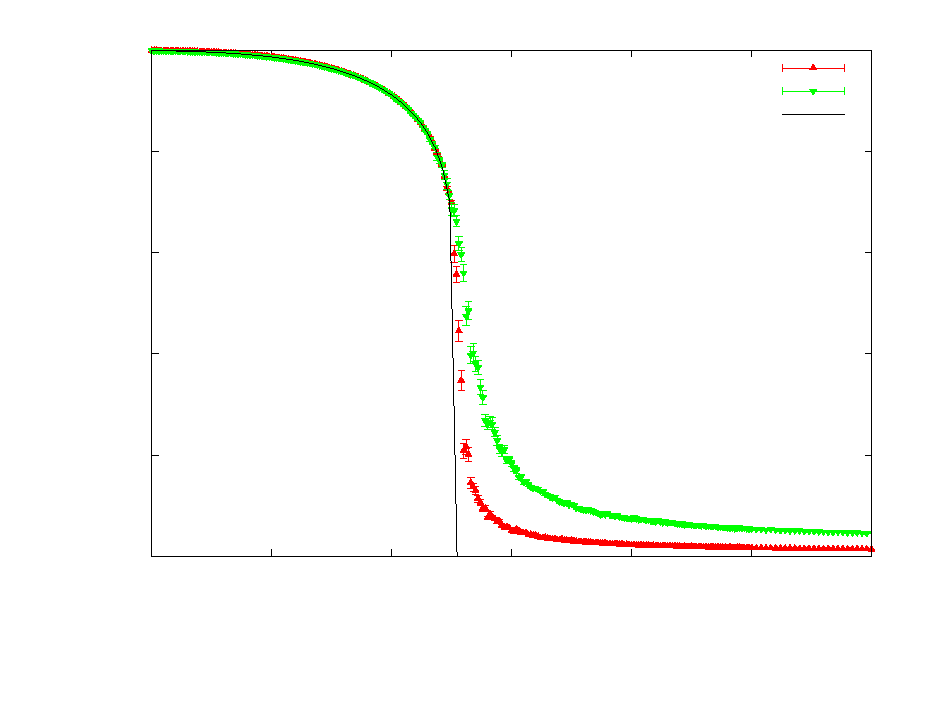
\includegraphics{magnetisierunglaenge}}%
    \gplfronttext
  \end{picture}%
\endgroup

		\caption[Magnetisierung bei verschiedenen Längen]{Magnetisierung bei verschiedenen Längen, Fehler gemessen mit Blocklänge 128}
		\label{fig:maglaenge}
	\end{figure}

	\begin{figure}[htbp]
		% GNUPLOT: LaTeX picture with Postscript
\begingroup
  \makeatletter
  \providecommand\color[2][]{%
    \GenericError{(gnuplot) \space\space\space\@spaces}{%
      Package color not loaded in conjunction with
      terminal option `colourtext'%
    }{See the gnuplot documentation for explanation.%
    }{Either use 'blacktext' in gnuplot or load the package
      color.sty in LaTeX.}%
    \renewcommand\color[2][]{}%
  }%
  \providecommand\includegraphics[2][]{%
    \GenericError{(gnuplot) \space\space\space\@spaces}{%
      Package graphicx or graphics not loaded%
    }{See the gnuplot documentation for explanation.%
    }{The gnuplot epslatex terminal needs graphicx.sty or graphics.sty.}%
    \renewcommand\includegraphics[2][]{}%
  }%
  \providecommand\rotatebox[2]{#2}%
  \@ifundefined{ifGPcolor}{%
    \newif\ifGPcolor
    \GPcolortrue
  }{}%
  \@ifundefined{ifGPblacktext}{%
    \newif\ifGPblacktext
    \GPblacktextfalse
  }{}%
  % define a \g@addto@macro without @ in the name:
  \let\gplgaddtomacro\g@addto@macro
  % define empty templates for all commands taking text:
  \gdef\gplbacktext{}%
  \gdef\gplfronttext{}%
  \makeatother
  \ifGPblacktext
    % no textcolor at all
    \def\colorrgb#1{}%
    \def\colorgray#1{}%
  \else
    % gray or color?
    \ifGPcolor
      \def\colorrgb#1{\color[rgb]{#1}}%
      \def\colorgray#1{\color[gray]{#1}}%
      \expandafter\def\csname LTw\endcsname{\color{white}}%
      \expandafter\def\csname LTb\endcsname{\color{black}}%
      \expandafter\def\csname LTa\endcsname{\color{black}}%
      \expandafter\def\csname LT0\endcsname{\color[rgb]{1,0,0}}%
      \expandafter\def\csname LT1\endcsname{\color[rgb]{0,1,0}}%
      \expandafter\def\csname LT2\endcsname{\color[rgb]{0,0,1}}%
      \expandafter\def\csname LT3\endcsname{\color[rgb]{1,0,1}}%
      \expandafter\def\csname LT4\endcsname{\color[rgb]{0,1,1}}%
      \expandafter\def\csname LT5\endcsname{\color[rgb]{1,1,0}}%
      \expandafter\def\csname LT6\endcsname{\color[rgb]{0,0,0}}%
      \expandafter\def\csname LT7\endcsname{\color[rgb]{1,0.3,0}}%
      \expandafter\def\csname LT8\endcsname{\color[rgb]{0.5,0.5,0.5}}%
    \else
      % gray
      \def\colorrgb#1{\color{black}}%
      \def\colorgray#1{\color[gray]{#1}}%
      \expandafter\def\csname LTw\endcsname{\color{white}}%
      \expandafter\def\csname LTb\endcsname{\color{black}}%
      \expandafter\def\csname LTa\endcsname{\color{black}}%
      \expandafter\def\csname LT0\endcsname{\color{black}}%
      \expandafter\def\csname LT1\endcsname{\color{black}}%
      \expandafter\def\csname LT2\endcsname{\color{black}}%
      \expandafter\def\csname LT3\endcsname{\color{black}}%
      \expandafter\def\csname LT4\endcsname{\color{black}}%
      \expandafter\def\csname LT5\endcsname{\color{black}}%
      \expandafter\def\csname LT6\endcsname{\color{black}}%
      \expandafter\def\csname LT7\endcsname{\color{black}}%
      \expandafter\def\csname LT8\endcsname{\color{black}}%
    \fi
  \fi
    \setlength{\unitlength}{0.0500bp}%
    \ifx\gptboxheight\undefined%
      \newlength{\gptboxheight}%
      \newlength{\gptboxwidth}%
      \newsavebox{\gptboxtext}%
    \fi%
    \setlength{\fboxrule}{0.5pt}%
    \setlength{\fboxsep}{1pt}%
\begin{picture}(8640.00,6480.00)%
    \gplgaddtomacro\gplbacktext{%
      \csname LTb\endcsname%
      \put(1164,1296){\makebox(0,0)[r]{\strut{}$-18$}}%
      \put(1164,1738){\makebox(0,0)[r]{\strut{}$-16$}}%
      \put(1164,2179){\makebox(0,0)[r]{\strut{}$-14$}}%
      \put(1164,2621){\makebox(0,0)[r]{\strut{}$-12$}}%
      \put(1164,3063){\makebox(0,0)[r]{\strut{}$-10$}}%
      \put(1164,3505){\makebox(0,0)[r]{\strut{}$-8$}}%
      \put(1164,3946){\makebox(0,0)[r]{\strut{}$-6$}}%
      \put(1164,4388){\makebox(0,0)[r]{\strut{}$-4$}}%
      \put(1164,4830){\makebox(0,0)[r]{\strut{}$-2$}}%
      \put(1164,5272){\makebox(0,0)[r]{\strut{}$0$}}%
      \put(1164,5713){\makebox(0,0)[r]{\strut{}$2$}}%
      \put(1164,6155){\makebox(0,0)[r]{\strut{}$4$}}%
      \put(1296,1076){\makebox(0,0){\strut{}$1$}}%
      \put(2448,1076){\makebox(0,0){\strut{}$1.5$}}%
      \put(3600,1076){\makebox(0,0){\strut{}$2$}}%
      \put(4752,1076){\makebox(0,0){\strut{}$2.5$}}%
      \put(5903,1076){\makebox(0,0){\strut{}$3$}}%
      \put(7055,1076){\makebox(0,0){\strut{}$3.5$}}%
      \put(8207,1076){\makebox(0,0){\strut{}$4$}}%
    }%
    \gplgaddtomacro\gplfronttext{%
      \csname LTb\endcsname%
      \put(526,3725){\rotatebox{-270}{\makebox(0,0){\strut{}$\dpd{M}{T}$}}}%
      \put(4751,746){\makebox(0,0){\strut{}Temperatur}}%
    }%
    \gplbacktext
    \put(0,0){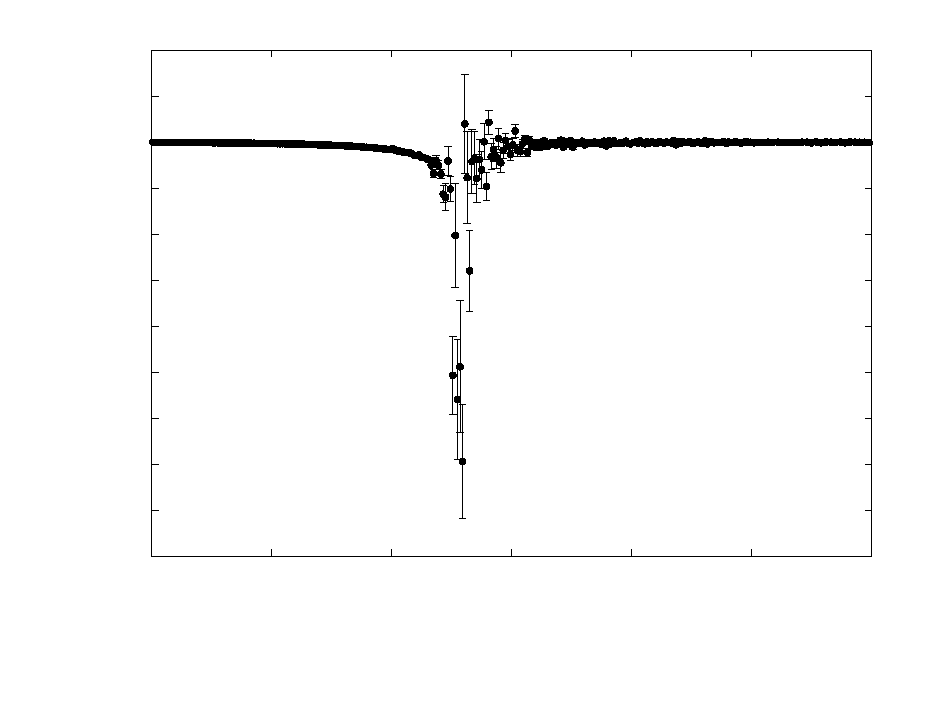
\includegraphics{ableitung120128}}%
    \gplfronttext
  \end{picture}%
\endgroup

		\caption[Ableitung der Magnetisierung]{Ableitung der Magnetisierung, berechnet mit Zwei-Punkt-Formel. Fehler mit Gaußscher Fehlerfortpflanzung aus den Fehlern bei Blocklänge 128 bestimmt}
		\label{fig:ableitung120128}
	\end{figure}
	
	In Bild \ref{fig:maglaenge} ist zusätzlich die nach Gl. \ref{eq:magnetisierungsgleichungliteratur} erwartete Magnetisierung eingezeichnet. Bis zum theoretischen kritischen Punkt, nach Gl. \ref{eq:kritischetemperatur} bei $T=\num{2,269}$, liegen alle Messdaten in ihren Fehlergrenzen auf der erwarteten Kurve, erst danach kommt es aufgrund des weniger starken Abfalls zu Abweichungen.
	
	Um den kritischen Punkt genauer zu bestimmen, wird zusätzlich mit der Zei-Punkt-Formel die Ableitung der gemessenen Magnetisierung bestimmt, siehe Bild \ref{fig:ableitung120128}. Dort wird sichtbar, dass die Änderungsrate der Magnetisierung meist sehr klein ist, nur um den kritischenb Punkt herum ist sie groß.% Die größte Änderung fand im Intervall $2,285\pm0,1$ statt, dies ist minimal größer als der theoretisch erwartete kritische Punkt, die Abweichung beträgt $1,5 \sigma$. 
%	Vergleich gemessene/theoretische Magnetisierung: Nur graphisch oder auch Rechnerisch: Anpassung an Bereich mit Fehlern != 0?
	%Größte Ableitung bei 2,285 pm 0,1 bei Länge 120.
	
	%Bestimmung kritischer Punkt? Über ableitung? Oder Kumulante wie in Binder/Herrmann?
	%Theoretischer Kritischer Punkt: J*2,269
%	Messungen mit QBiG, bei denen nur die Zeit zum Durchführen von 1000 Messungen bei verschiedenen Längen und mit verschieden vielen benutzten Kernen gemessen wurde, zeigen, dass bei kleinen Längen wie 10 die benötigte Zeit mit Anzahl der Kerne sogar zunimmt. Dies ist auf den Overhead zurückzuführen.
%		
%	
%	Messungen auf Intel(R) Core(TM) i7-7500U CPU @ 2.70GHz, lcpunode01 und lcpunode02 auf QBiG.